% !TEX root = ./xstream.tex

\section{Static evaluation}

\begin{table}[h!]
	\centering
	\begin{tabular}{lccc}
	\toprule
	\textbf{Dataset} & \textbf{Number of samples} & \textbf{Dimensionality} & \textbf{Number of Anomalies}\\
	\midrule
	\multicolumn{4}{c}{\textit{High-dimensional Datasets}}\\
	gisette 		& 7000 & 4970 & 3500	\\
	isolet 			& 7797 & 616 & 3300	\\
	letter			& 7797 & 616 & 3600	\\
	madelon 		& 2600 & 500 & 1300	\\
	\midrule
	\multicolumn{4}{c}{\textit{Low/medium-dimensional Datasets}}\\
	cancer 			& 568      & 30  & 211	\\
	ionosphere  & 350      & 33  & 125		\\
	telescope   & 19020    & 10  & 	6688		\\
	indians    	& 768      & 8	& 269		\\
	\bottomrule
	\end{tabular}
	\caption{Datasets used for the static evaluation.}
	\label{table:datasets}
\end{table}

\subsection{Datasets}

The datasets used are listed in Table \ref{table:datasets} to generate the subsequent datasets used in the static evaluation. They were chosen based on (TODO: selection logic).

\subsection{Generating anomalies for static evaluation}

We used 2 different procedures to generate the datasets on which to benchmark, one for the low/medium dimensional datasets and one for the high-dimensional datasets. They are described below:
\begin{enumerate}
	\item \textit{Approach 1:} We append new columns containing Gaussian noise to the original dataset, thereby increasing its dimensionality with noisy features. The number of noisy features is quantified as a percentage of the original dataset dimensionality. If the original dataset mean and standard deviation are $\mu$ and $\sigma$, the noisy columns contained Gaussian noise with mean $\rho\mu$ and standard deviation $\rho\sigma$, where $\rho$ is the noise factor. We consider appending 100\%, 1000\%, 2000\% and 5000\% noisy features, and use $\rho \in \{0.01, 0.1, 0.2, 0.25\}$.

	\item \textit{Approach 2:} We first discard all the original anomalous points. Now for the remaining nominal points, we first choose 10\% of the features at random and mark them as important features. We further proceed with choosing 5\% of the samples at random as important samples. Now, in this sub-block, which contains only important samples and important features, we add Gaussian noise to the original data. Again, Gaussian noise is used, parameterized by the mean, and the standard deviation of the entire nominal dataset. Further this noise is scaled according to the user-specified signal to noise ratio, and added to the original sub-block of our dataset and features.
\end{enumerate}

\pagebreak

\subsection{Competing methods and hyperparameter settings}

\textbf{XStream (XS)} was used with $K=100$ projections, $C=100$ chains and depth $d=15$. We implemented and compared against the following competing methods and parameter settings:

\begin{itemize}
	\item \textbf{iForest (IF)}: We use it with recommended sample size of $256$ or the entire dataset, whichever is minimum. The \texttt{hlim} is set to $15$ to be comparable to HS-Trees, and number of components is set to $100$.

	\item \textbf{HS-Trees (HST)}:  Use it with the recommended setting of $15$ max-depth and $100$ trees.

	\item \textbf{LODA}: We set the sparsity factor to $\frac{1}{\sqrt(d)}$. We allow LODA to select best width for histograms, but fix the number of histograms to $100$.

	\item \textbf{RS-Hash (RSH)}: We use $1000$ sampling points and $100$ components.
\end{itemize}

\subsection{Baseline Results}

Table \ref{table:static-results} lists the average precision of XStream and the competing methods on the generated datasets.
%A Friedman test for differences in the best-performing method across all datasets rejected the null hypothesis that the difference ranking between methods is not statistically significant with $p=2.2\times10^{-16} < 0.05$.

We conduct our experiments on datasets mentioned in Table~\ref{table:datasets}. A Friedman test for differences in the best-performing method across all datasets rejected the null hypothesis that the difference rankings between methods is not statistically significant with $p=0.0072 < 0.05$.

Hence, we perform a posthoc-Friedman test, Nemenyi test to compare all methods to each other. We first compute average ranks of all the methods over the  $8$ original datasets, which is shown in Table~\ref{table:OriginalRanks}. Setting significance level to be $\alpha=0.05$, we get the $q_{0.05}$ for $k=5$ pairs as $2.728$. Difference in average ranks of any two methods will be significant if 
\begin{align}
(R_{i} - R_{j}) > q_{\alpha} \sqrt{\frac{k(k+1)}{6N}}
\end{align}
Setting $N=8$ and $k=5$, for difference between a pair of methods to be significant, the difference between the rank should be greater than $2.1567$. Looking at the average ranks shown in Table~\ref{table:OriginalRanks}, we can say the (X-Stream, LODA) and (X-Stream, I-Forest) are significantly different.

To show the effect of adding high-dimensionality, we add noisy columns to the $4$ original datasets. The noise is generated as mentioned above in Approach 1. The average ranks for all the methods is shown in Table~\ref{table:LowDimRanks}. Using Friedman test, we can reject the null hypothesis that the difference rankings between methods is not statistically significant with $p=3.451\times 10^{-10}$. We again perform posthoc-Friedman Nemenyi test; setting $N=16$ and $k=5$, we obtain that difference in average ranks should be greater than $1.524$. Observing the table, we find difference to be significant between (LODA, I-Forest), (X-Stream, I-Forest), (LODA, HS-Trees), (X-Stream, HS-Trees) and (X-Stream, RS-Hash).

%Wilcoxon signed-rank test to compare methods pairwise and obtain a ranking over all datasets. Table \ref{table:wilcoxon-all} contains $p$-values from the Wilcoxon signed-rank test. Each cell $(i,j)$ in the table contains the $p$-value of the hypothesis that method $i$ has a higher AP than method $j$ is statistically significant. Hence, \textbf{XS} > \textbf{LODA} > \textbf{RSH} > \textbf{IF} > \textbf{HST} is statistically significant at $p=0.05$

\begin{table}
	\centering
    \begin{tabular}{llllll}
    	\toprule
               & IF         & HST        & RSH        & LODA       & XS          \\	\hline
    cancer     & 0.635(5.0) & 0.758(3.0) & 0.719(4.0) & 0.883(2.0) & 0.9035(1.0) \\
    ionosphere & 0.819(4.0) & 0.824(3.0) & 0.83(2.0)  & 0.79(5.0)  & 0.8952(1.0) \\
    telescope  & 0.655(3.0) & 0.674(2.0) & 0.678(1.0) & 0.623(5.0) & 0.6339(4.0) \\
    indians    & 0.498(4.0) & 0.502(3.0) & 0.518(2.0) & 0.48(5.0)  & 0.5382(1.0) \\
    gisette    & 0.423(4.0) & 0.417(5.0) & 0.432(3.0) & 0.436(2.0) & 0.4424(1.0) \\
    isolet     & 0.442(4.0) & 0.444(2.5) & 0.444(2.5) & 0.429(5.0) & 0.4445(1.0) \\
    letter     & 0.475(2.0) & 0.453(5.0) & 0.471(3.0) & 0.46(4.0)  & 0.4865(1.0) \\
    madelon    & 0.501(5.0) & 0.507(4.0) & 0.511(3.0) & 0.515(2.0) & 0.5277(1.0) \\	\midrule
    AVG RANK   & 3.875      & 3.4375     & 2.5625     & 3.75       & 1.375       \\
    \bottomrule
    \end{tabular}
    \caption {Average rank of methods over the 8 original datasets}
            \label{table:OriginalRanks}

\end{table}

%\begin{figure*}[ht!]
%    \centering
%        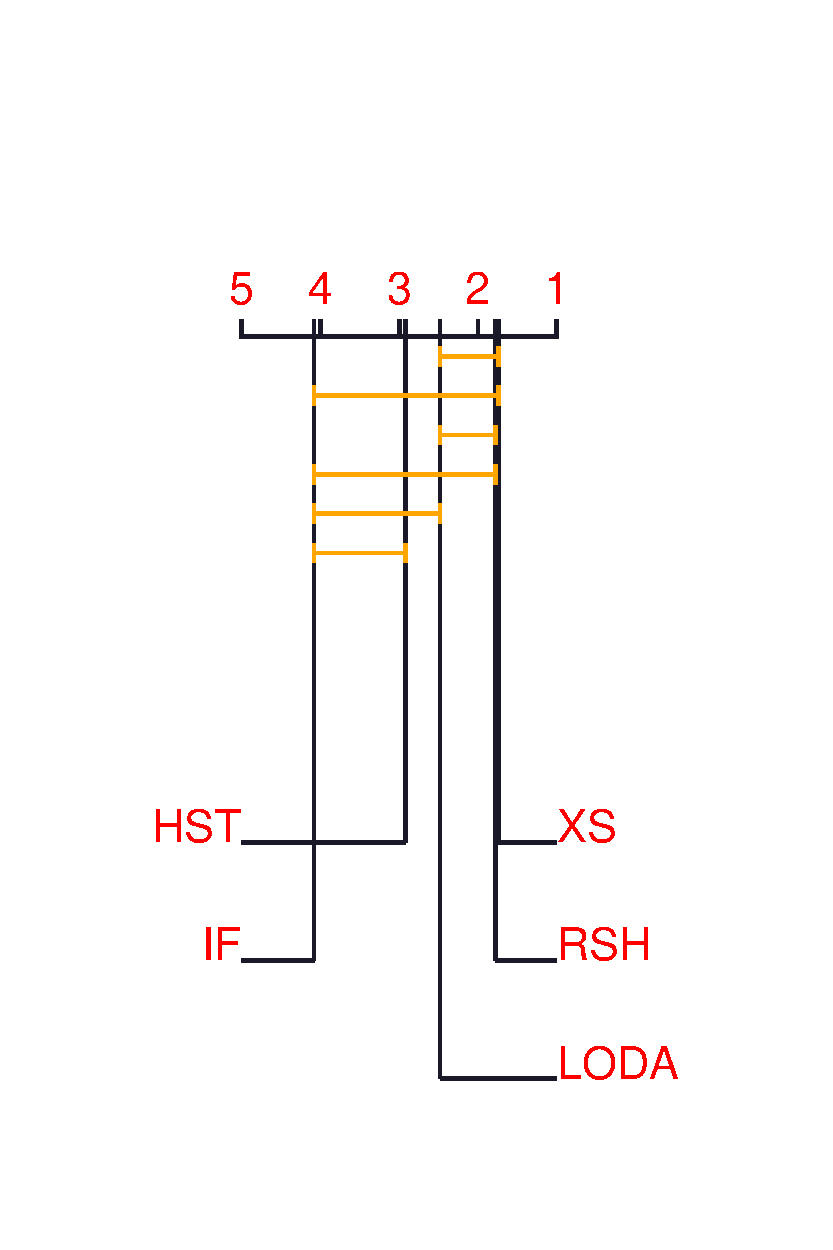
\includegraphics[scale=0.3]{fig/Neyemi_LowDim.pdf}
%        \caption{Low/Mid - dimensional dataset analysis. Significance is shown via the connected lines.}
%\end{figure*}

%\begin{figure*}[ht!]
%    \centering
%        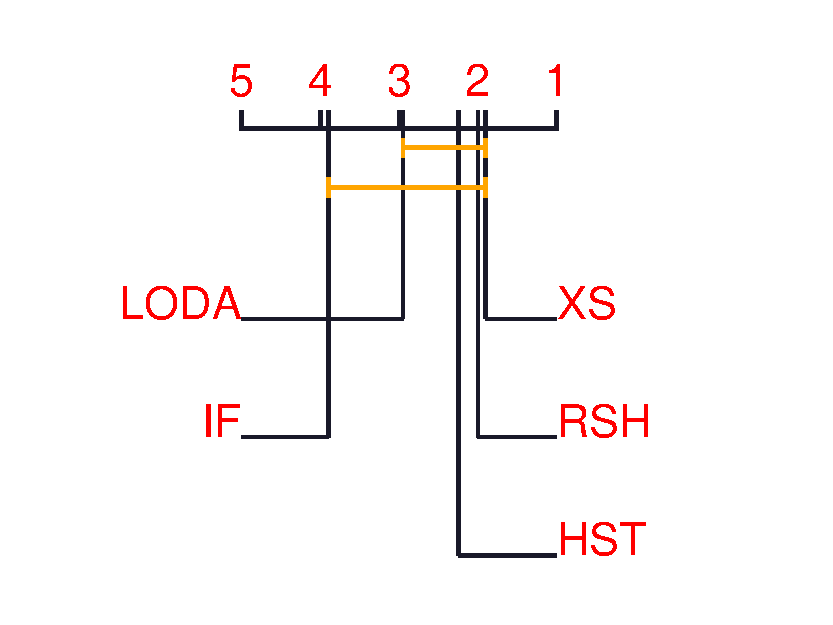
\includegraphics[scale=0.3]{fig/Neyemi_Overall_Original.pdf}
%        \caption{All original dataset - neyemeni test  - Significance is shown via the connected lines.}
%\end{figure*}

\begin{table}
	\centering
    \begin{tabular}{llllll}
    \toprule
               & IF         & HST        & RSH        & LODA       & XS          \\	\hline
    cancer100      & 0.661(5.0) & 0.727(3.0) & 0.702(4.0) & 0.839(2.0) & 0.8511(1.0) \\
    cancer1000     & 0.476(4.0) & 0.394(5.0) & 0.531(3.0) & 0.686(2.0) & 0.8453(1.0) \\
    cancer2000     & 0.447(4.0) & 0.444(5.0) & 0.474(3.0) & 0.643(2.0) & 0.8282(1.0) \\
    cancer5000     & 0.404(4.0) & 0.4(5.0)   & 0.425(3.0) & 0.508(2.0) & 0.7729(1.0) \\
    ionosphere100  & 0.756(4.0) & 0.773(2.0) & 0.725(5.0) & 0.771(3.0) & 0.9005(1.0) \\
    ionosphere1000 & 0.59(3.0)  & 0.573(5.0) & 0.579(4.0) & 0.742(2.0) & 0.8706(1.0) \\
    ionosphere2000 & 0.441(5.0) & 0.505(3.0) & 0.446(4.0) & 0.736(2.0) & 0.8743(1.0) \\
    ionosphere5000 & 0.403(3.0) & 0.376(5.0) & 0.399(4.0) & 0.675(2.0) & 0.7966(1.0) \\
    telescope100   & 0.593(4.0) & 0.576(5.0) & 0.601(3.0) & 0.617(2.0) & 0.6373(1.0) \\
    telescope1000  & 0.451(4.0) & 0.419(5.0) & 0.471(3.0) & 0.592(2.0) & 0.6095(1.0) \\
    telescope2000  & 0.407(4.5) & 0.407(4.5) & 0.409(3.0) & 0.586(2.0) & 0.5872(1.0) \\
    telescope5000  & 0.376(5.0) & 0.38(3.0)  & 0.378(4.0) & 0.538(2.0) & 0.5752(1.0) \\
    indians100     & 0.477(3.0) & 0.444(5.0) & 0.478(2.0) & 0.472(4.0) & 0.5218(1.0) \\
    indians1000    & 0.385(4.0) & 0.379(5.0) & 0.397(3.0) & 0.444(2.0) & 0.4976(1.0) \\
    indians2000    & 0.35(5.0)  & 0.361(4.0) & 0.369(3.0) & 0.41(2.0)  & 0.4777(1.0) \\
    indians5000    & 0.343(4.0) & 0.338(5.0) & 0.349(3.0) & 0.4(2.0)   & 0.4659(1.0) \\	\hline
    AVG. Rank              & 4.09375    & 4.3475     & 3.375      & 2.1875     & 1           \\    \bottomrule
    \end{tabular}
    \caption {Average rank of methods over the 16 perturbed datasets.}
        \label{table:LowDimRanks}
\end{table}



%Hence, we perform a Wilcoxon signed-rank test to compare methods pairwise and obtain a ranking over all datasets. Table \ref{table:wilcoxon-all} contains $p$-values from the Wilcoxon signed-rank test. Each cell $(i,j)$ in the table contains the $p$-value of the hypothesis that method $i$ has a higher AP than method $j$ is statistically significant. Hence, \textbf{XS} > \textbf{LODA} > \textbf{RSH} > \textbf{IF} > \textbf{HST} is statistically significant at $p=0.05$.
%\begin{table}[h!]
%		\centering
%    \begin{tabular}{lllllll}
%    \toprule
%    ~        & \textbf{IF}   & \textbf{RSH}    & \textbf{LODA}      & \textbf{HST}  & \textbf{XS} \\
%		\midrule
%    \textbf{IF}  	 & ---       			& 0.9870    		& 0.9727   			& \textbf{0.0194}   						& 0.9989       \\
%    \textbf{RSH}   & \textbf{0.0135} 	& ---       		& 0.9542   			& $\pmb{6.7540\times10^{-5}}$ & 0.9981       \\
%    \textbf{LODA}  & \textbf{0.0282} 	& 0.0471    		& ---      			& 0.0003   							& 0.9999      \\
%    \textbf{HST} 	 & 0.9812    			& 0.9999    		& 0.9997   			& ---         					& 1.0000       \\
%    \textbf{XS}    & \textbf{0.0012} & \textbf{0.0020} & \textbf{0.0001} & $\pmb{2.0490\times10^{-5}}$  & ---       \\
%		\bottomrule
%    \end{tabular}
%    \caption{$p$-values from a Wilcoxon signed-rank test on the average precisions reported on all the datasets. Bold values are significant at $p=0.05$. Each cell $(i,j)$ contains the $p$-value of the hypothesis that method $i$ has a greater AP than method $j$. It can be observed that \textbf{XS} > \textbf{LODA} > \textbf{RSH} > \textbf{IF} > \textbf{HST} is statistically significant at $p=0.05$.}
%		\label{table:wilcoxon-all}
%\end{table}
%
%When repeated on just the high-dimensional datasets, we can conclude that \textbf{RS} > \textbf{LODA}, \textbf{RS} > \textbf{HST} and \textbf{IF} > \textbf{HST} at $p=0.05$. We do not have enough evidence to make enough comparisons to construct a total order among methods.

% \begin{table}[]
% \centering
% \begin{tabular}{l|lll}
% \hline	\hline
% \textbf{Friedman Statistic} & \textbf{Low-Dim Datasets} & \textbf{High-Dim Datasets} & \textbf{All Datasets}    \\ \hline
% p-value            & 1.155e-09        & 8.362e-10         & \textless2.2e-16 \\ \hline \hline
% \textbf{Wilcoxon Test}      & \multicolumn{3}{c}{\textbf{p-val w/ XST}}                        \\ 	\hline
% iFor               & 1.907e-06         & 0.7271         &  0.001196       \\
% RSH                & 6.676e-06         & 0.7392         & 0.002026        \\
% LODA               & 9.537e-07         & 0.1744         & 0.0001096            \\
% HSTrees            & 2.861e-06        & 0.2375          &  2.049e-05	\\	\hline
% \end{tabular}
% \caption{Friedman's test statistics among methods. And wilcoxon test p-values, indicating that XStream performs better than all the baseline methods for low-dimensional datasets and over the set of all datasets, but no method is more significant than XStream and vice-versa.}
% \label{my-label}
% \end{table}

% \begin{table}
% \centering
%     \begin{tabular}{|l|lllll|}
%     \hline
%        & IF        & HST       & RSH      & LODA      & XS \\	\hline
%    IF   & ~         & 0.4839    & 0.9999   & 0.9977    & 1  \\
%    HST  & 0.5321    & ~         & 0.9999   & 0.9299    & 1  \\
%    RSH  & 0.0001307 & 0.0001049 & ~        & 0.0001974 & 1  \\
%    LODA & 0.002552  & 0.07526   & 0.9998   & ~         & 1  \\
%    XS   & 1.91E-06  & 2.86E-06  & 9.54E-07 & 6.68E-06  & ~  \\
%    \hline
%\end{tabular}
%     \caption{Wilcoxon test p-value result for Low Dimension dataset. XST > RSH > LODA > HST $\sim$ IF}
% \end{table}
%
% \begin{table}
% \centering
%     \begin{tabular}{|l|lllll|}
%     \hline
%      & IF     & HST       & RSH    & LODA    & XS     \\	\hline
%    IF   & ~      & 0.006183  & 0.7432 & 0.07528 & 0.2853 \\
%    HST  & 0.9944 & ~         & 0.9999 & 0.7996  & 0.7738 \\
%    RSH  & 0.2689 & 0.0001156 & ~      & 0.02964 & 0.2729 \\
%    LODA & 0.9299 & 0.211     & 0.9728 & ~       & 0.835  \\
%    XS   & 0.7271 & 0.2375    & 0.7392 & 0.1744  & ~      \\
%    \hline
%    \end{tabular}
%     \caption{Wilcoxon test p-value result for High Dimension dataset. IF > HST, RSH > HST, RSH > LODA}
% \end{table}
%
% \begin{table}
% \centering
%     \begin{tabular}{|l|lllll|}
%     \hline
%     & IF        & HST      & RSH       & LODA      & XS     \\	\hline
%    IF   & ~         & 0.01942  & 0.987     & 0.9727    & 0.9989 \\
%    HST  & 0.9812    & ~        & 0.999     & 0.997     & 1      \\
%    RSH  & 0.0135    & 6.75E-05 & ~         & 0.9542    & 0.9981 \\
%    LODA & 0.0001096 & 0.02815  & 0.0003357 & 0.04711   & 0.9999 \\
%    XS   & 0.001196  & 2.05E-05 & 0.002026  & 0.0001096 & ~      \\    \hline
%\end{tabular}
%     \caption{Wilcoxon test p-value result for all datasets. XS > LODA > RSH > IF > HST}
% \end{table}

%\begin{table}
%\centering
%    \begin{tabular}{l|llll}
%         & IF        & HST       & RSH       & LODA      \\	\hline
%    HST  & 0.095377  & ~         & ~         & ~         \\
%    ~    & 0.462     & ~         & ~         & ~         \\
%    RSH  & -2.346292 & -2.44167  & ~         & ~         \\
%    ~    & 0.0095*   & 0.0073*   & ~         & ~         \\
%    LODA & -0.305208 & -0.400586 & 2.041084  & ~         \\
%    ~    & 0.3801    & 0.3444    & 0.0206*   & ~         \\
%    XS   & -3.657055 & -3.752433 & -1.310762 & -3.351846 \\
%    ~    & 0.0001*   & 0.0001*   & 0.095     & 0.0004*   \\
%    \end{tabular}
%    \caption{Bonferonni-Dunn test for Low dimensional datasets}
%\end{table}
%
%\begin{table}
%\centering
%    \begin{tabular}{l|llll}
%         & IF       & HST       & RSH      & LODA      \\	\hline
%    HST  & 1.158165 & ~         & ~        & ~         \\
%    ~    & 0.1234   & ~         & ~        & ~         \\
%    RSH  & 0.035426 & -1.122739 & ~        & ~         \\
%    ~    & 0.4859   & 0.1308    & ~        & ~         \\
%    LODA & 0.951058 & -0.207107 & 0.915631 & ~         \\
%    ~    & 0.1708   & 0.418     & 0.1799   & ~         \\
%    XS   & 0.771201 & -0.386963 & 0.735775 & -0.179856 \\
%    ~    & 0.2203   & 0.3494    & 0.2309   & 0.4286    \\
%    \end{tabular}
%    \caption{Bonferonni-Dunn test for High dimensional datasets}
%\end{table}
%
%\begin{table}
%\centering
%    \begin{tabular}{l|llll}
%         & IF        & HST       & RSH       & LODA      \\	\hline
%    HST  & 0.835458  & ~         & ~         & ~         \\
%    ~    & 0.2017    & ~         & ~         & ~         \\
%    RSH  & -0.129423 & -0.964882 & ~         & ~         \\
%    ~    & 0.4485    & 0.1673    & ~         & ~         \\
%    LODA & -0.826765 & -1.662224 & -0.697342 & ~         \\
%    ~    & 0.2042    & 0.0482    & 0.2428    & ~         \\
%    XS   & -1.622624 & -2.458083 & -1.493201 & -0.795858 \\
%    ~    & 0.0523    & 0.0070*   & 0.0677    & 0.2131    \\
%    \end{tabular}
%    \caption{Bonferonni-Dunn test for ALL datasets}
%\end{table}

%\begin{table}
%\centering
%    \begin{tabular}{l|llll}
%         & IF       & HST      & RSH     & LODA    \\	\hline
%    HST  & 0.99998  & -        & -       & -       \\
%    RSH  & 0.02638  & 0.03543  & -       & -       \\
%    LODA & 0.34478  & 0.40322  & 0.80663 & -       \\
%    XS   & 4.90E-08 & 8.90E-08 & 0.03061 & 0.00061 \\
%    \end{tabular}
%    \caption {Post Friedman - Nemeneyi Test - Low Dim Datasets}
%\end{table}
%
%\begin{table}
%\centering
%    \begin{tabular}{l|llll}
%         & IF    & HST   & RSH   & LODA  \\	\hline
%    HST  & 0.129 & -     & -     & -     \\
%    RSH  & 0.982 & 0.031 & -     & -     \\
%    LODA & 0.266 & 0.997 & 0.08  & -     \\
%    XS   & 0.957 & 0.465 & 0.722 & 0.691 \\
%    \end{tabular}
%    \caption{Post Friedman - Nemeneyi Test - High Dim Datasets}
%\end{table}
%
%\begin{table}
%\centering
%    \begin{tabular}{l|llll}
%         & IF     & HST      & RSH    & LODA   \\	\hline
%    HST  & 0.5031 & -        & -      & -      \\
%    RSH  & 0.4357 & 0.0089   & -      & -      \\
%    LODA & 0.9625 & 0.1571   & 0.8438 & -      \\
%    XS   & 0.0025 & 1.70E-06 & 0.2937 & 0.0248 \\
%    \end{tabular}
%     \caption{Post Friedman - Nemeneyi Test - ALL Datasets}
%\end{table}


\begin{footnotesize}
\begin{table}[p!]
    %\centering
		\begin{tabular}{lcccccc}
				\toprule
				\textbf{Dataset} & \textbf{IF} &  \textbf{HST} & \textbf{RSH} &  \textbf{LODA}  & \textbf{XS}\\
				\midrule
				\multicolumn{6}{c}{\textit{High-dimensional Datasets}}\\
%gisette& $0.423 \pm 0.011$ &  $0.417 \pm 0.005$ &  $0.432 \pm 0.017$ &  $0.436 \pm 0.008$ &  $0.4424 \pm 0.0081$    \\
gisette(30,0.3,1.2 )& $0.683 \pm 0.045$ &  $0.46 \pm 0.005$ &  $0.628 \pm 0.021$ &  $0.531 \pm 0.018$ &  $0.5282 \pm 0.0091$    \\
gisette (30,0.3,10.0 )& $0.541 \pm 0.027$ &  $0.354 \pm 0.002$ &  $0.471 \pm 0.024$ &  $0.321 \pm 0.004$ &  $0.3204 \pm 0.0029$    \\
gisette (30,0.3,20.0 )& $0.45 \pm 0.022$ &  $0.308 \pm 0.003$ &  $0.347 \pm 0.017$ &  $0.29 \pm 0.003$ &  $0.292 \pm 0.0032$    \\
gisette (30,0.3,30.0 )& $0.432 \pm 0.016$ &  $0.31 \pm 0.002$ &  $0.316 \pm 0.006$ &  $0.301 \pm 0.005$ &  $0.2929 \pm 0.0023$    \\
%gisette (30,0.3,50.0 )& $0.408 \pm 0.009$    \\
isolet& $0.442 \pm 0.019$ &  $0.444 \pm 0.001$ &  $0.444 \pm 0.013$ &  $0.429 \pm 0.02$ &  $0.4445 \pm 0.0067$    \\
\midrule
isolet (30,0.3,1.2 )& $0.537 \pm 0.03$ &  $0.441 \pm 0.01$ &  $0.559 \pm 0.028$ &  $0.58 \pm 0.03$ &  $0.6396 \pm 0.0204$    \\
isolet (30,0.3,10.0 )& $0.372 \pm 0.011$ &  $0.334 \pm 0.004$ &  $0.391 \pm 0.015$ &  $0.35 \pm 0.007$ &  $0.3479 \pm 0.0066$    \\
isolet (30,0.3,20.0 )& $0.33 \pm 0.009$ &  $0.311 \pm 0.001$ &  $0.322 \pm 0.007$ &  $0.313 \pm 0.006$ &  $0.3176 \pm 0.0017$    \\
isolet (30,0.3,30.0 )& $0.3 \pm 0.002$ &  $0.296 \pm 0.001$ &  $0.293 \pm 0.002$ &  $0.292 \pm 0.004$ &  $0.2899 \pm 0.0016$    \\
%isolet (30,0.3,50.0 )& $0.313 \pm 0.003$    \\
\midrule
%letter& $0.475 \pm 0.012$ &  $0.453 \pm 0.003$ &  $0.471 \pm 0.009$ &  $0.46 \pm 0.011$ &  $0.4865 \pm 0.0075$    \\
letter (30,0.3,1.2 )& $0.49 \pm 0.026$ &  $0.44 \pm 0.01$ &  $0.519 \pm 0.053$ &  $0.534 \pm 0.03$ &  $0.5967 \pm 0.0204$    \\
letter (30,0.3,10.0 )& $0.374 \pm 0.015$ &  $0.339 \pm 0.008$ &  $0.375 \pm 0.007$ &  $0.337 \pm 0.003$ &  $0.3361 \pm 0.005$    \\
letter (30,0.3,20.0 )& $0.309 \pm 0.008$ &  $0.291 \pm 0.002$ &  $0.31 \pm 0.007$ &  $0.289 \pm 0.002$ &  $0.3 \pm 0.0015$    \\
letter (30,0.3,30.0 )& $0.319 \pm 0.01$ &  $0.308 \pm 0.001$ &  $0.307 \pm 0.004$ &  $0.305 \pm 0.003$ &  $0.3095 \pm 0.0023$    \\
%letter (30,0.3,50.0 )& $0.307 \pm 0.002$    \\
\midrule
%madelon& $0.501 \pm 0.008$ &  $0.507 \pm 0.003$ &  $0.511 \pm 0.01$ &  $0.515 \pm 0.014$ &  $0.5277 \pm 0.008$    \\
madelon (5,0.05,1.2 )& $0.896 \pm 0.051$ &  $0.92 \pm 0.007$ &  $0.969 \pm 0.039$ &  $1.0 \pm 0.0$ &  $1.0 \pm 0.0$    \\
madelon (5,0.05,10.0 )& $0.643 \pm 0.13$ &  $0.784 \pm 0.068$ &  $0.899 \pm 0.094$ &  $0.988 \pm 0.012$ &  $0.9567 \pm 0.023$    \\
madelon (5,0.05,20.0 )& $0.24 \pm 0.093$ &  $0.16 \pm 0.039$ &  $0.377 \pm 0.143$ &  $0.112 \pm 0.027$ &  $0.125 \pm 0.0133$    \\
madelon (5,0.05,30.0 )& $0.07 \pm 0.013$ &  $0.083 \pm 0.004$ &  $0.099 \pm 0.059$ &  $0.054 \pm 0.007$ &  $0.0444 \pm 0.0034$    \\
%madelon (5.0,0.05,50.0 )& $0.051 \pm 0.004$    \\
\midrule
\multicolumn{6}{c}{\textit{Low/medium-dimensional Datasets}}\\
%breast-cancer-wisconsin& $0.635 \pm 0.024$ &  $0.758 \pm 0.004$ &  $0.719 \pm 0.019$ &  $0.883 \pm 0.019$ &  $0.9035 \pm 0.0104$    \\
cancer (100,0.1 )& $0.661 \pm 0.036$ &  $0.727 \pm 0.01$ &  $0.702 \pm 0.026$ &  $0.839 \pm 0.024$ &  $0.8511 \pm 0.0216$    \\
cancer (1000,0.1 )& $0.476 \pm 0.043$ &  $0.394 \pm 0.007$ &  $0.531 \pm 0.047$ &  $0.686 \pm 0.047$ &  $0.8453 \pm 0.0179$    \\
cancer (2000,0.1 )& $0.447 \pm 0.026$ &  $0.444 \pm 0.015$ &  $0.474 \pm 0.046$ &  $0.643 \pm 0.066$ &  $0.8282 \pm 0.0212$    \\
cancer (5000,0.1 )& $0.404 \pm 0.021$ &  $0.4 \pm 0.013$ &  $0.425 \pm 0.022$ &  $0.508 \pm 0.086$ &  $0.7729 \pm 0.0394$    \\
\midrule
%ionosphere& $0.819 \pm 0.008$ &  $0.824 \pm 0.003$ &  $0.83 \pm 0.005$ &  $0.79 \pm 0.014$ &  $0.8952 \pm 0.0084$    \\
ionosphere (100,0.1 )& $0.756 \pm 0.031$ &  $0.773 \pm 0.005$ &  $0.725 \pm 0.018$ &  $0.771 \pm 0.013$ &  $0.9005 \pm 0.0052$    \\
ionosphere (1000,0.1 )& $0.59 \pm 0.044$ &  $0.573 \pm 0.008$ &  $0.579 \pm 0.054$ &  $0.742 \pm 0.032$ &  $0.8706 \pm 0.01$    \\
ionosphere (2000,0.1 )& $0.441 \pm 0.033$ &  $0.505 \pm 0.033$ &  $0.446 \pm 0.027$ &  $0.736 \pm 0.029$ &  $0.8743 \pm 0.0052$    \\
ionosphere (5000,0.1 )& $0.403 \pm 0.022$ &  $0.376 \pm 0.006$ &  $0.399 \pm 0.028$ &  $0.675 \pm 0.048$ &  $0.7966 \pm 0.0117$    \\
\midrule
%magic-telescope& $0.655 \pm 0.011$ &  $0.674 \pm 0.003$ &  $0.678 \pm 0.005$ &  $0.623 \pm 0.004$ &  $0.6339 \pm 0.0061$    \\
telescope (100,0.1 )& $0.593 \pm 0.01$ &  $0.576 \pm 0.005$ &  $0.601 \pm 0.015$ &  $0.617 \pm 0.003$ &  $0.6373 \pm 0.0077$    \\
telescope (1000,0.1 )& $0.451 \pm 0.018$ &  $0.419 \pm 0.008$ &  $0.471 \pm 0.021$ &  $0.592 \pm 0.013$ &  $0.6095 \pm 0.0054$    \\
telescope (2000,0.1 )& $0.407 \pm 0.021$ &  $0.407 \pm 0.003$ &  $0.409 \pm 0.018$ &  $0.586 \pm 0.007$ &  $0.5872 \pm 0.0087$    \\
telescope (5000,0.1 )& $0.376 \pm 0.011$ &  $0.38 \pm 0.002$ &  $0.378 \pm 0.005$ &  $0.538 \pm 0.026$ &  $0.5752 \pm 0.0074$    \\
\midrule
%pima-indians& $0.498 \pm 0.015$ &  $0.502 \pm 0.005$ &  $0.518 \pm 0.006$ &  $0.48 \pm 0.015$ &  $0.5382 \pm 0.0052$    \\
indians (100,0.1 )& $0.477 \pm 0.013$ &  $0.444 \pm 0.009$ &  $0.478 \pm 0.007$ &  $0.472 \pm 0.01$ &  $0.5218 \pm 0.0077$    \\
indians (1000,0.1 )& $0.385 \pm 0.017$ &  $0.379 \pm 0.006$ &  $0.397 \pm 0.024$ &  $0.444 \pm 0.014$ &  $0.4976 \pm 0.0106$    \\
indians (2000,0.1 )& $0.35 \pm 0.014$ &  $0.361 \pm 0.005$ &  $0.369 \pm 0.023$ &  $0.41 \pm 0.016$ &  $0.4777 \pm 0.0082$    \\
indians (5000,0.1 )& $0.343 \pm 0.008$ &  $0.338 \pm 0.003$ &  $0.349 \pm 0.014$ &  $0.4 \pm 0.028$ &  $0.4659 \pm 0.009$    \\
				\bottomrule
		\end{tabular}
		\caption{Average precision of static methods on high-dimensional (top) and low/medium-dimensional (bottom) datasets. Mean and standard deviation reported over 10 runs. Numbers in the brackets indicate: (top) the percentage of features, fraction of samples to which noise is added, signal-to-noise ratio, and (bottom) noise column amount (as $\%$ of original dimensionality), relative noise factor.}
		\label{table:static-results}
\end{table}
\end{footnotesize}


\begin{footnotesize}
\begin{table}[!hbtp]
		\begin{tabular}{lcccccc}
		\toprule
		\textbf{Dataset} & \textbf{IF} &  \textbf{HST} & \textbf{RSH} &  \textbf{LODA}  & \textbf{XS}\\
		\midrule
				\multicolumn{6}{c}{\textit{Original Datasets}}\\
		gisette& $0.423 \pm 0.011$ &  $0.417 \pm 0.005$ &  $0.432 \pm 0.017$ &  $0.436 \pm 0.008$ &  $0.4424 \pm 0.0081$    \\
		isolet& $0.442 \pm 0.019$ &  $0.444 \pm 0.001$ &  $0.444 \pm 0.013$ &  $0.429 \pm 0.02$ &  $0.4445 \pm 0.0067$    \\
		letter& $0.475 \pm 0.012$ &  $0.453 \pm 0.003$ &  $0.471 \pm 0.009$ &  $0.46 \pm 0.011$ &  $0.4865 \pm 0.0075$    \\
		madelon& $0.501 \pm 0.008$ &  $0.507 \pm 0.003$ &  $0.511 \pm 0.01$ &  $0.515 \pm 0.014$ &  $0.5277 \pm 0.008$    \\
		cancer& $0.635 \pm 0.024$ &  $0.758 \pm 0.004$ &  $0.719 \pm 0.019$ &  $0.883 \pm 0.019$ &  $0.9035 \pm 0.0104$    \\
		ionosphere& $0.819 \pm 0.008$ &  $0.824 \pm 0.003$ &  $0.83 \pm 0.005$ &  $0.79 \pm 0.014$ &  $0.8952 \pm 0.0084$    \\
		telescope& $0.655 \pm 0.011$ &  $0.674 \pm 0.003$ &  $0.678 \pm 0.005$ &  $0.623 \pm 0.004$ &  $0.6339 \pm 0.0061$    \\
		indians& $0.498 \pm 0.015$ &  $0.502 \pm 0.005$ &  $0.518 \pm 0.006$ &  $0.48 \pm 0.015$ &  $0.5382 \pm 0.0052$    \\
		\bottomrule
		\end{tabular}
		\caption{Average precision of static methods on original, unperturbed datasets. Mean and standard deviation are reported over 10 runs.}
\end{table}
\end{footnotesize}

\subsection{Time and Space Complexity}
%
%

\begin{table}[h!]
	\caption{Symbol List}
	\centering
	\begin{tabular}{lll}
		\toprule
		\textbf{Symbols} & \textbf{Description}	\\	\hline
		$N$ & Number of data points	\\	\hline
		$D$ & Number of dimensions/features	\\	\hline
		$C$ & Number of ensemble components (trees, chains, histograms, etc.)	\\	\hline
		$d$ & Max depth of trees/chains	\\	\hline
		$\psi$ & iForest/HS-Trees/RS-Hash: sampling size	\\	\hline
		$r$ & RS-Hash: Number of sampled dimensions	\\
		$b$ & LODA: number of histogram bins	\\	\hline
		$m$ & \method/RS-Hash: Number of CMS hash functions	\\
		$L$ & \method/RS-Hash:: CMS hash table size	\\	\hline
		$k$ & \method: Number of random projections	\\
		$M$ & \method: Number of subspaces	\\
		$W$ & \method: Number of windows	\\
		\bottomrule
	\end{tabular}
\end{table}

\begin{table}[h!]
	\caption{Time and space complexity of the ensemble anomaly detection algorithms compared in this paper.
		In streaming case, a data point/vector arrives at a time for HS-Stream, LODA, and RS-Hash; whereas
		an update to a single feature for a data point arrives at a time.}

	\centering
	\begin{tabular}{l|lclcl}
		\toprule
		\textbf{Algorithm} & \multicolumn{2}{l}{\textbf{Time Complexity}} &&& \textbf{Space Complexity}	\\
		& \multicolumn{3}{l}{\noindent\rule[0.5ex]{0.5\linewidth}{1pt}}
		& &  \multicolumn{1}{l}{\noindent\rule[0.5ex]{0.2\linewidth}{1pt}} \\
		& Training && Scoring/Updating && \\\hline
		{\em Batch/Offline} &&& & & \\
		iForest & $O(C\psi \log \psi)$ & & $O(C \log \psi)$ &  & $O(C\psi)$	\\
		HS-Trees & $O(Cd\psi)$ & &$O(Cd)$ && $O(C2^d)$ \\
		LODA & $O(NC\sqrt{D})$  & & $O(C\sqrt{D})$  && $O(C\sqrt{D} + Cb)$ \\
		RS-Hash & $O(Crm\psi)$ & & $O(Crm)$ && $O(CLm)$\\
		\method & $O(M[NDk + Ckmd])$ & &$O(M[Dk + Ckmd])$ && $O(MCLmd)$   \\
		\hline
		{\em Streaming/Online}  & & &&& \\
		HS-Stream & \multicolumn{1}{c}{--} & & $O(Cd + C\psi)$ && $O(C2^d)$ \\
		LODA & \multicolumn{1}{c}{--} & &$O(C\sqrt{D} + Cb)$ && $O(C\sqrt{D} + Cb)$\\
		RS-Hash & \multicolumn{1}{c}{--} & & $O(Crm)$ && $O(CLm)$\\
		\method & \multicolumn{1}{c}{--} & & $O(WMCkmd)$  && $O(WMCLmd)$   \\
		\bottomrule
	\end{tabular}
\end{table}

\subsection{Running time}

iForest is the fastest, RSHash is the slowest (RSHash implementation, however can be optimized)
\begin{figure*}[ht!]
    \centering
    \begin{subfigure}[t]{0.48\textwidth}
        \centering
        \includegraphics[width=\linewidth]{fig/baseline/TimeAnalysis_LowDim.png}
        \caption{Low/Mid - dimensional dataset analysis}
    \end{subfigure}
    \hfill
    \begin{subfigure}[t]{0.48\textwidth}
        \centering
        \includegraphics[width=\linewidth]{fig/baseline/TimeAnalysis_HighDim.pdf}
        \caption{High dimensional dataset analysis}
    \end{subfigure}
		\hfill
    \caption{RunTimes of algorithms over datasets with different noise levels. X-axis is over different datasets with different noise levels. Y-axis is log of runtime (in seconds).}
\end{figure*}

\pagebreak
